\documentclass{article}
\usepackage[utf8]{inputenc}
\usepackage[portuguese]{babel}
\usepackage[a4paper, total={7in, 9in}]{geometry}
\usepackage{graphicx}
\usepackage{float}
\usepackage{verbatim}
\usepackage[bottom]{footmisc}
\usepackage[style=numeric]{biblatex}
\usepackage{minted}
\usepackage{csquotes}
\usepackage{fancyvrb}
\usepackage[title]{appendix}
\usepackage{xcolor}
\usepackage{indentfirst}
\addbibresource{references.bib}

\newcommand{\titleRule}{
    \rule{\linewidth}{0.5mm} \\ [0.25cm]
}

\begin{document}

{
\center
\textsc{\Large Universidade do Minho} \\ [0.5cm]
\textsc{\Large Mestrado Integrado em Engenharia Informática} \\ [0.5cm]
\textsc{\large Scripting no Processamento de Linguagem Natural} \\ [0.5cm]

{\LARGE \bfseries Spell Checker} \\[0.2cm]

\begin{tabular}{c c}
    Diana Ribeiro Barbosa & José Carlos Lima Martins \\
    A78679 & A78821  \\
\end{tabular} \\[0.5cm]

\today \\[1cm]
}

\tableofcontents

\section{Introdução}
O presente trabalho foi desenvolvido no âmbito da unidade curricular Scripting no Processamento de Linguagem Natural, do perfil de especialização Processamento de Linguagens e Conhecimento do 4º ano do Mestrado Integrado em Engenharia Informática da Universidade do Minho.
\par O objetivo do mesmo é criação de uma ferramenta para Processamento de Linguagem Natural, neste caso, uma ferramenta que possibilite a correção de erros ortográficos em textos escritos em português de Portugal.
\par Assim, ao longo deste relatório fazemos uma análise ao problema, explicamos a solução que desenvolvemos, como proceder à sua utilização (com o auxílio de exemplos práticos), como instalar bem como enumeramos as conclusões a que chegamos e algumas ideias que gostaríamos de futuramente implementar no projeto.

\section{Análise do Problema}\label{prob}

No vocabulário da língua portuguesa de Portugal existem várias palavras que se escrevem de forma semelhante diferindo apenas numa letra, símbolo e/ou espaço o que leva muitas vezes a erros ortográficos quando são escritas. Este é o caso de palavras homófonas cuja pronúncia é igual mas que se escrevem de forma diferente (e.g. "\textit{à}" e "\textit{há}") e dos casos "tracinho se".

O objetivo deste trabalho prático consiste na criação de uma ferramenta que permita a correção ortográfica de erros do tipo "tracinho se", isto é, dado um texto \textit{input} com erros gramaticais deste tipo, é esperado que o programa devolva como resultado uma versão do texto na qual se encontram corrigidos todos os erros de "tracinho se" que encontrar. No entanto, optamos pela criação de uma ferramenta que seja versátil o suficiente de modo que consiga corrigir vários tipos de erros ortográficos, nomeadamente o exemplo já referido de "\textit{há vs à}", bastando apenas especificar quais os tipos de erros que se pretende corrigir.

%%%%%%%%%%%%%%%%%%%%%%%%%%%%%%%%%%%%%%%%%%%%%%%
\section{Solução desenvolvida}
Do processo de desenho e conceção da solução para o problema em mãos, exposto na secção \ref{prob}, resultou uma aplicação capaz de corrigir erros ortográficos dos mais diversos tipos. Segue-se a explicação do funcionamento dos dois componentes principais em que se divide, nomeadamente, a construção do dicionário de \textit{n-grams} e a correção ortográfica do texto \textit{input}.

\subsection{Construção do dicionário de \textit{n-grams}}
A aplicação desenvolvida, tal como explicado previamente, tem como objetivo a correção de erros ortográficos num dado texto. De modo a conseguir alcançar este objetivo foi necessário perceber a maneira mais adequada de o fazer, isto é, como dar ao programa conhecimento suficiente para que este consiga efetuar as correções necessárias de forma correta. Posto isto, acabamos por optar pela utilização de \textit{n-grams}, concretamente, a criação de um dicionário de \textit{n-grams} a partir de um dado \textit{corpus}. Convém assim explicar ambos os conceitos. Um \textit{n-gram}, no contexto de processamento de linguagens, é uma sequência de n elementos contíguos num dado texto\cite{ngram}. Quanto ao segundo conceito, um \textit{corpus} linguístico é uma coletânia de textos escritos e registos orais numa determinada língua\cite{corpus}, neste caso, português de Portugal. 

Voltando à explicação da solução, decidimos que a melhor implementação seria a criação de um dicionário (a partir de um dado \textit{corpus}) que contivesse todos os \textit{n-grams} desse tamanho lá presentes bem como, para cada um deles, o seu respetivo número de ocorrências. Assim, o programa irá possuir inúmeros exemplos de palavras escritas corretamente e o contexto em que se inserem a que poderá recorrer para verificar, num dado texto \textit{input}, se uma certa palavra está bem escrita tendo em conta o seu contexto. A título de exemplo, suponhamos a expressão "\textit{À oito dias que não como}" que possui um erro ortográfico no uso do "\textit{à}" ao invés do "\textit{há}". A ferramenta consulta o dicionário para conseguir encontrar a parte da expressão que preveja este caso (com n-grams de um tamanho especificado) e, caso encontre, verifica que é muito mais provável que a palavra correta para esta expressão seja "\textit{há}" e procede à substituição, devolvendo como resultado "\textit{Há oito dias que não como}".

Quanto ao \textit{corpus} utilizado, usamos o CetemPUBLICO (Corpus de Extractos de Textos Electrónicos MCT/ Público), um \textit{corpus} de aproximadamente 180 milhões de palavras em português europeu retiradas do jornal português "Público"\cite{jornal}. No entanto, foi necessário um pré-processamento dos dados uma vez que os textos não estavam prontos a ser usados (i.e. prontos para a construção do dicionário). Assim, criamos um script em \texttt{awk} (\texttt{convert.awk}) para a remoção das anotações de modo a restarem apenas as palavras e símbolos normais do texto

\begin{verbatim}
        $0 !~ /^<\/?([spta]|ext|mwe).*?/ {printf "%s ", $1}
\end{verbatim}

e um script para a conversão do \textit{encoding} do texto de \texttt{ISO-8859-1} para \texttt{UTF-8}.

\begin{verbatim}
        #!/bin/bash

        FROM_ENCODING="ISO-8859-1"
        TO_ENCODING="UTF-8"
        CONVERT="iconv -f $FROM_ENCODING -t $TO_ENCODING"
        
        for  file  in  *.txt; do
             $CONVERT   "$file"   -o  "${file%.txt}.utf8.txt"
        done
        exit 0
\end{verbatim}

De seguida, após a conversão para \texttt{UTF-8}, aplicamos o script em \texttt{awk} para cada um dos textos do \textit{corpus} (através do ficheiro \texttt{getText.sh}).

\begin{verbatim}
        #!/bin/bash
        for  file  in  *.txt; do
             gawk -f convert.awk "$file" > "${file%.utf8.txt}.txt"
        done
        exit 0
\end{verbatim}

Por fim, juntou-se todos os textos para um único ficheiro através de:

\begin{verbatim}
        cat CETEMPublicoAnotado2009.000.txt CETEMPublicoAnotado2009.001.txt 
            CETEMPublicoAnotado2009.002.txt CETEMPublicoAnotado2009.003.txt 
                                        ... 
            CETEMPublicoAnotado2009.221.txt CETEMPublicoAnotado2009.222.txt 
            CETEMPublicoAnotado2009.223.txt > CETEMPublicoAnotado2009.txt
\end{verbatim}

Para poder utilizar os dicionários do \textit{corpus} CetemPUBLICO (disponibilizamos para n-grams de tamanho 2 e 3) basta ir à diretoria \texttt{ngrams\_dict} e proceder à sua instalação conforme indicado (processo em detalhe na secção \ref{usage}). Caso o utilizador pretenda utilizar qualquer outro \textit{corpus}, pode-o fazer através da opção \texttt{-b} bastando especificar o ficheiro que contém o corpus e o tamanho dos \textit{n-grams} a serem criados. Em ambos os casos, os dicionários são guardados em \texttt{~/.pickle} com o nome \texttt{spellcheck-pt-words-X.pkl}, sendo \texttt{X} o tamanho dos n-gramas lá guardados.

Por fim, convém ainda referir que antes e após a criação dos n-grams (com a opção \texttt{-b}) é chamado o \textit{garbage collector} do Python por forma a tentar reduzir o consumo de memória (RAM).


\subsection{Correção ortográfica}
Uma vez tendo os dicionários necessários ao exemplos que se pretende aplicar, entra a componente da verificação ortográfica. Primeiramente, é necessário especificar que tipo de erros se pretende corrigir (e.g. erros de "tracinho se"). Esta especificação é feita no ficheiro \texttt{configfile}. Este deve seguir a seguinte configuração: 

\begin{itemize}
    \item Em cada linha existem quatro campos divididos por "\texttt{ ||| }".
    \item Os dois primeiros campos contêm os erros que se pretendem corrigir, nomeadamente, as suas alternativas (e.g. "-se" e "sse").
    \item O terceiro campo contém a expressão regular (padrão) que representa os caracteres imediatamente antes do possível erro.
    \item O quarto campo contém a expressão regular (padrão) que representa os caracteres imediatamente depois do possível erro.
    \item Apenas os dois primeiros campos são de preenchimento obrigatório.
    \item Para verificar um novo tipo de erro basta acrescentar uma nova linha ao \texttt{configfile} com a sua especificação seguindo as presentes regras sintáticas.
\end{itemize}

\begin{figure}[H]
\begin{center}
    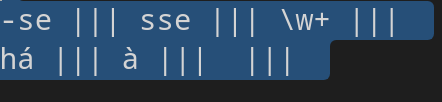
\includegraphics[width = 6cm, keepaspectratio]{Pictures/cf.png}
    \caption{Exemplo de especificação correta do ficheiro \texttt{configfile}. }
\end{center}
\end{figure}

Caso o ficheiro esteja mal formado e como tal possua erros sintáticos, é devolvida a seguinte mensagem de erro.

\begin{figure}[H]
\begin{center}
    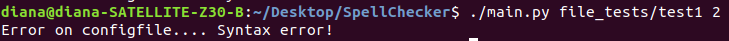
\includegraphics[width = 16cm, keepaspectratio]{Pictures/errocf.png}
    \caption{Mensagem de erro resultante de uma especificação incorreta do ficheiro \texttt{configfile}. }
\end{center}
\end{figure}

Quanto ao processo de verificação ortográfica o primeiro passo é percorrer as linhas do \texttt{configfile} para sabermos que tipos de erro queremos verificar. Para cada linha do ficheiro, criamos dois regex's com os valores dessa linha, sendo que os regex's são criados tendo em conta se os terceiro e quarto campos (da linha do ficheiro de configuração que está a ser analisada) existem. Isto é importante para conseguir fazer as substituições corretamente e de forma simples, uma vez que são adicionados grupos de captura ao regex para os campos 3 (padrão que precede o que queremos verificar) e 4 (padrão que sucede o que queremos verificar).

De seguida, são percorridas todas as palavras do texto input (sem os símbolos e sem os caracteres de espaçamento) e para cada palavra verificamos se faz match com algum dos regex's criados. Caso isto aconteça, se fizer com o primeiro chamamos a função \texttt{sub} para o primeiro caso do \texttt{configfile}, caso contrário chamamos sub para o segundo caso do \texttt{configfile}.

A função \texttt{sub}, primeiramente cria os \textit{n-grams} para um caso (primeiro caso se houver match com o 1º regex anteriormente referido e segundo caso se for com o 2º regex) do \texttt{configfile}, ou seja, vê as palavras contíguas e gera apenas os \textit{n-grams} a que ela pertence (e.g. na frase "\textit{Andou em direção há saída da estação}", caso tenham sido especificados pelo utilizador n-gramas de tamanho 2, a função sub criará para a verificação de "há", os n-gramas "direção há" e "há saída"). Em segundo lugar, são obtidos os valores da ocorrência desses n-gramas no dicionário de n-grams carregado relativo a esse tamanho e é feito o somatório do número dessas ocorrências. Por fim, é repetido o processo para o caso contrário, isto é, o segundo campo da linha de configuração ser a opção correta (se primeiramente foi feito para o primeiro campo) ou o primeiro campo da linha de configuração ser a opção correta (se primeiramente foi feito para o segundo campo). Concretamente, são calculados os n-gramas, obtidos os valores de ocorrência e feita a soma dos mesmos.

O ultimo passo deste processo é a comparação dos somatórios das ocorrências. Aquele que for maior é considerado o caso correto. Caso haja um empate, mantém-se a palavra original, caso contrário substitui-se na lista de palavras (do texto criada inicialmente). Convém ainda referir que todo este processo é repetido para cada linha do ficheiro de configuração, portanto, para um \texttt{config file} com duas linhas o texto input é percorrido duas vezes.

Por fim, resta a recuperação do texto na qual se substituem todas as palavras do backup inicialmente feito ao texto input pelas "novas", ou seja, apenas não são alterados os símbolos e os espaços do texto original.



%%%%%%%%%%%%%%%%%%%%%%%%%%%%%%%%%%%%%%%%%%%%%%%
\section{Utilização}\label{usage}
No que toca à utilização da aplicação, para uma maior facilidade de uso, criamos o seguinte menu de ajuda que pode ser acedido através de \verb|./main.py -h|, sendo o output o seguinte:

\begin{verbatim}
        Usage: ./main.py [OPTIONS] [FILENAME] [N-GRAM-SIZE]
        Default behaviour: output spell checked file content
        
        Options:
          -b	Build n-grams dictionary
          -o	Output filename of default behaviour
          -h	Help
        
        Example: ./main.py text.txt 2

\end{verbatim}

Como é possível constatar através da observação do menu de ajuda, a nossa aplicação oferece quatro opções distintas de funcionamento, nomeadamente:
\begin{enumerate}
    \item Verificação ortográfica de um dado texto com n-grams de um dado tamanho (\textit{default}).
    \item Verificação ortográfica de um dado texto com n-grams de um dado tamanho, sendo o resultado guardado num ficheiro (onde o utilizador escolhe o nome).
    \item Criação do dicionário de n-grams a partir de um corpus escolhido pelo utilizador.
    \item Menu de ajuda.
\end{enumerate}

Passamos agora a explicar cada uma delas em mais detalhe.

\paragraph{Verificação ortográfica de um dado texto com n-grams de um dado tamanho (\textit{default}):} 
A funcionalidade em questão é o funcionamento \textit{default} da aplicação, não sendo portanto necessária nenhuma \textit{flag} para a sua utilização. Neste caso, o utilizador indica o nome do ficheiro que contém o texto que se pretende corrigir, bem como o tamanho de n-grams a utilizar. Como resultado temos a versão corrigida do texto \textit{input} que é imprimida no terminal, como se pode verificar pela imagem abaixo.

\begin{figure}[H]
\begin{center}
    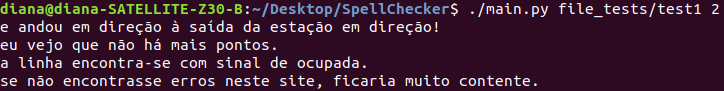
\includegraphics[width = 16cm, keepaspectratio]{Pictures/default.png}
    \caption{Exemplo do funcionamento \textit{default}. }
\end{center}
\end{figure}

\paragraph{Verificação ortográfica de um dado texto com n-grams de um dado tamanho, sendo o resultado guardado num ficheiro (onde o utilizador escolhe o nome):} 
Esta funcionalidade é bastante semelhante à anterior na medida em que devolve como resultado o texto \textit{input} com as correções ortográficas necessárias. No entanto, neste caso o utilizador para além da \textit{flag} (\texttt{-o}) indica também o nome de um ficheiro no qual será guardado o resultado, ao invés deste ser imprimido no terminal como na opção \textit{default}. Na imagem abaixo podemos ver um exemplo no qual é usada a opção \texttt{-o} e, imediatamente a seguir a este, temos a indicação do nome de um ficheiro (\texttt{output.txt}). Como é possível verificar, nenhum resultado foi imprimido no terminal e vendo o conteúdo de \texttt{output.txt} encontramos lá a versão corrigida do texto input, tal como pretendido.

\begin{figure}[H]
\begin{center}
    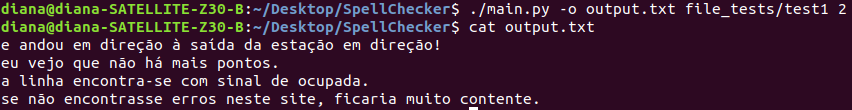
\includegraphics[width = 16cm, keepaspectratio]{Pictures/o.png}
    \caption{Exemplo do funcionamento com a \textit{flag} \texttt{-o}. }
\end{center}
\end{figure}

\paragraph{Criação do dicionário de n-grams a partir de um corpus escolhido pelo utilizador:} 
Esta funcionalidade tem como objetivo permitir ao utilizador a utilização de um corpus à sua escolha. Para tal, o utilizador deve indicar o nome do ficheiro que contém o corpus bem como o tamanho dos n-grams a serem criados. Deste modo, será criado o dicionário (de n-grams e as suas respetivas ocorrências) de acordo com a especificação fornecida e em futuras utilizações, até indicação em contrário, será este o dicionário a que o programa recorre. Convém referir que caso se crie um dicionário para um dado tamanho x que já exista (a partir de um corpus indicado pelo utilizador), é substituído o existente pelo novo. Para além disso, caso o utilizador tente verificar um texto com um tamanho de n-grams para o qual não possui um dicionário, o programa não irá funcionar. Concretamente, nestes casos, surge uma mensagem de erro que indica a ausência de um dicionário para esse tamanho e como proceder para o criar.

\begin{figure}[H]
\begin{center}
    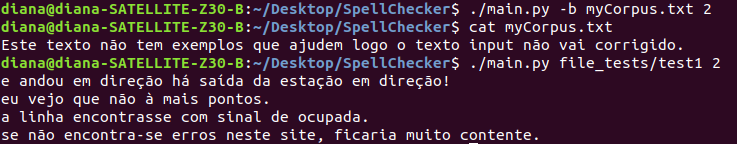
\includegraphics[width = 16cm, keepaspectratio]{Pictures/b.png}
    \caption{Exemplo do funcionamento com a \textit{flag} \texttt{-b}. }
\end{center}
\end{figure}

\begin{figure}[H]
\begin{center}
    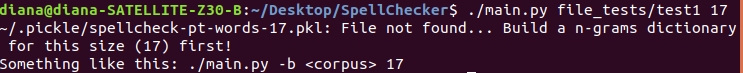
\includegraphics[width = 16cm, keepaspectratio]{Pictures/erro.png}
    \caption{Exemplo de erro de ausência de dicionário para o tamanho indicado dos n-grams. }
\end{center}
\end{figure}

\paragraph{Menu de ajuda:} Por fim, a última opção quanto ao funcionamento do programa é a utilização da \textit{flag} \texttt{-h} da qual se obtém o menu de ajuda. Este indica como usar a aplicação, as opções que estão disponíveis, qual o comportamento \textit{default} do programa e ainda um exemplo de utilização. 

\section{Instalação}

Como já referimos previamente, a aplicação exige a existência de um corpus para a correção de um determinado texto. Deste modo, o utilizador pode criar os seus dicionários de n-grams através da flag \texttt{-b} com o seu corpus ou usar os dicionário de n-grams disponibilizados que usaram como corpus o CETEMPublicoAnotado2009. Por forma a usar os dicionários de n-grams disponibilizados o utilizador deve proceder à instalação dos mesmos ao realizar os seguintes passos:

\begin{itemize}
    \item Fazer \textit{unzip} dos ficheiros:
\end{itemize}

\begin{verbatim}
        cat spellcheck-pt-words-2.pkl.gz_aa spellcheck-pt-words-2.pkl.gz_ab 
            spellcheck-pt-words-2.pkl.gz_ac spellcheck-pt-words-2.pkl.gz_ad 
            > spellcheck-pt-words-2.pkl.gz
        
        gunzip spellcheck-pt-words-2.pkl.gz
        
        cat spellcheck-pt-words-3.pkl.gz_aa spellcheck-pt-words-3.pkl.gz_ab 
            spellcheck-pt-words-3.pkl.gz_ac spellcheck-pt-words-3.pkl.gz_ad 
            spellcheck-pt-words-3.pkl.gz_ae spellcheck-pt-words-3.pkl.gz_af 
            spellcheck-pt-words-3.pkl.gz_ag spellcheck-pt-words-3.pkl.gz_ah 
            spellcheck-pt-words-3.pkl.gz_ai spellcheck-pt-words-3.pkl.gz_aj 
            spellcheck-pt-words-3.pkl.gz_ak spellcheck-pt-words-3.pkl.gz_al 
            > spellcheck-pt-words-3.pkl.gz
        
        gunzip spellcheck-pt-words-3.pkl.gz
\end{verbatim}


\begin{itemize}
    \item Criar a pasta pickle:
\end{itemize}

\begin{verbatim}
        mkdir ~/.pickle
\end{verbatim}

\begin{itemize}
    \item Mover dicionários de n-grams para a pasta pickle:
\end{itemize}

\begin{verbatim}
        mv spellcheck-pt-words-2.pkl spellcheck-pt-words-3.pkl ~/.pickle
\end{verbatim}


Concluídos estes passos e após a instalação do \texttt{python3} no sistema onde será utilizado o programa, o programa encontra-se pronto a ser utilizado.

\section{Conclusões e Trabalho Futuro}

Após a realização deste trabalho surgiram-nos algumas ideias que consideramos interessantes e que gostaríamos de implementar futuramente. Em primeiro lugar, expandir a ferramenta de modo a fazer as verificações ortográficas para um número elevado de erros sendo que para tal é apenas necessário acrescentar esses casos ao ficheiro \texttt{configfile}, o que é uma grande mais-valia da aplicação, no caso, a sua versatilidade.

Em segundo lugar, manter nas substituições das palavras a capitalização do texto inicial, o que de momento não está a acontecer. Isto é, após a verificação ortográfica de todo o texto este sofre uma substituição de cada uma das suas palavras que foram previamente guardadas em letra minúscula, ou seja, não são só as palavras corrigidas que são substituídas no texto original. Deste modo, o texto perde toda a sua capitalização, sendo este um ponto que gostaríamos de ver resolvido.

Por outro lado, seria possível expandir a ferramenta numa outra direção, concretamente, correção de erros semânticos. Isto seria possível recorrendo à \textit{framework} estudada no trabalho prático anterior, concretamente, o \textit{Polyglot} devido às suas funcionalidades de análise da categoria de palavras (e.g. advérbio) entre outras.

A nível de conclusões a que chegamos, no que toca ao funcionamento da aplicação, apercebemo-nos de que o tamanho mais adequado e eficiente para os n-grams é 2, uma vez que dado um corpus (sobre o qual se constrói o dicionário de n-grams e o número das suas ocorrências) quanto maior o tamanho de cada n-gram, mais particular é esse caso e menor a probabilidade de ocorrer (i.e. a probabibilidade de ocorrer num texto um dado n-gram diminui conforme o número de palavras deste aumenta). Assim, utilizar um dicionário de n-grams de tamanho dois melhora a capacidade de corrigir com sucesso um texto versus utilizar um dicionário de tamanho 3 (para o mesmo corpus) já que é mais provável os n-grams do texto input existirem no dicionário de tamanho 2 do que no de tamanho 3. No entanto, convém referir que apesar dos contras já mencionados, a utilização de n-grams maiores tem como prós uma maior confiança na correção já que analisa melhor o contexto em que a palavra está inserida e confere um maior grau de certeza a cada correção.

Por fim, consideramos que a realização deste trabalho nos permitiu desenvolver pensamento crítico bem como conhecimentos na área de Scripting e de Processamento de Linguagens em geral. A nível do trabalho desenvolvido, fazemos uma apreciação positiva do mesmo e acreditamos ter superado os objetivos uma vez que a aplicação é capaz de corrigir não só erros do tipo "tracinho se" como pedido, mas também uma grande variedade deles (sendo que exemplificamos para o caso "à versus há").


\printbibliography

\newpage 
\begin{appendices}

\end{appendices}

\end{document} 